\documentclass[aspectratio=169,xcolor=dvipsnames]{beamer}
% 1. Definir el color ANTES de llamar al tema SimplePlus
\usepackage{xcolor}
\definecolor{nyugray}{RGB}{128,128,128}
\usetheme{SimplePlus}
\definecolor{UnalGreen}{RGB}{0,153,51}
\usepackage[utf8]{inputenc}
\usepackage[spanish]{babel}
\deactivatequoting
\usepackage{hyperref}
\usepackage{graphicx}
\usepackage{booktabs}
\usepackage{tikz}
\usepackage{pgfplots}
% NOTA: no se declara \pgfplotsset{compat=...} a propósito (ver convenciones del curso)
\usetikzlibrary{positioning, arrows.meta, calc}
\usepackage[skip=5pt]{caption}
\captionsetup{justification=justified, font=small}
\usefonttheme{professionalfonts}

% ----- PLACEHOLDER PARA IMÁGENES EXTERNAS -----
\newcommand{\imgwarning}[2][0.8]{%
	\begin{center}
		\fcolorbox{nyugray}{gray!8}{%
			\parbox[c][3.2cm][c]{#1\textwidth}{\centering\small\textcolor{nyugray}{%
					[\,Insertar imagen: #2\,]}}%
		}
	\end{center}
}

\title{Fundamentos de Mecánica -- Taller}
\subtitle{Sesión 4: Movimiento Circular}
\titlegraphic{%
	\vspace*{-0.3cm}%
	\IfFileExists{imagenes/universidad-nacional-de-colombia-sede-bogota-seeklogo.png}{%
		\includegraphics[width=2.2cm]{imagenes/universidad-nacional-de-colombia-sede-bogota-seeklogo.png}%
	}{%
		\IfFileExists{universidad-nacional-de-colombia-sede-bogota-seeklogo.png}{%
			
\includegraphics[width=2.2cm]{universidad-nacional-de-colombia-sede-bogota-seeklogo.png}%
		}{}%
	}%
	\hspace{1.0cm}%
	\IfFileExists{logoMIAI_white.png}{%
		
\includegraphics[width=4.0cm]{logoMIAI_white.png}%
	}{%
		\IfFileExists{imagenes/logoMIAI_white.png}{%
			\includegraphics[width=4.0cm]{imagenes/logoMIAI_white.png}%
		}{}%
	}%
}
\author{Miguel Andrés Perdomo Gutiérrez}
\institute{%
	Auxiliar Docente | M.Sc. en Ciencias -- Física\\
	Universidad Nacional de Colombia -- Sede Bogotá
}
\date{25 de septiembre de 2026}

\begin{document}
	
	% ============================================================
	% SLIDE 1: PORTADA
	% ============================================================
	\begin{frame}
		\titlepage
	\end{frame}
	
	% ============================================================
	% SLIDE 2: AGENDA DE LA SESIÓN
	% ============================================================
	\begin{frame}{Agenda de la Sesión}
		\centering
		\begin{tikzpicture}[
			box/.style={rectangle, rounded corners, draw=UnalGreen, thick, fill=UnalGreen!10,
				minimum width=2.4cm, minimum height=1.9cm, align=center, font=\small},
			arr/.style={-{Latex[length=2mm]}, thick, UnalGreen}
			]
			\node[box] (b1) {Sustentación\\Taller 3\\(Cinemática 2D)\\\textbf{50 min}};
			\node[box, right=0.5cm of b1] (b2) {Socialización\\y cierre\\\textbf{10 min}};
			\node[box, right=0.5cm of b2] (b3) {Movimiento\\Circular\\\textbf{55 min}};
			\node[box, right=0.5cm of b3] (b4) {Preguntas\\y dudas\\\textbf{5 min}};
			\draw[arr] (b1) -- (b2);
			\draw[arr] (b2) -- (b3);
			\draw[arr] (b3) -- (b4);
		\end{tikzpicture}
		
		\vspace{0.5cm}
		\begin{itemize}
			\item Duración total: \textbf{2 horas} (Viernes 09:00--11:00, Edificio 401, Salón 202).
			\item Primera parte: sustentación en tablero del Taller 3 (Cinemática 2D: tiro parabólico y movimiento circular paramétrico).
			\item Segunda parte: Movimiento Circular -- coordenadas polares, velocidad y aceleración angular.
		\end{itemize}
	\end{frame}
	
	% ============================================================
	% SLIDE 3: SUSTENTACIÓN TALLER 3
	% ============================================================
	\begin{frame}{Sustentación Taller 3: Cinemática 2D}
		\begin{itemize}
			\item Se sortea, uno a uno, \textbf{un grupo} y luego \textbf{un integrante} de ese grupo para sustentar un ejercicio del Taller 3 en el tablero.
			\item Retroalimentación inmediata de toda la clase después de cada sustentación.
			\item Se repite el sorteo hasta evaluar a todos los grupos (o hasta agotar el tiempo asignado).
		\end{itemize}
		\begin{alertblock}{Recordatorio}
			Si un grupo no es sorteado, su nota corresponde a la revisión del procedimiento escrito (memoria grupal) entregado al inicio de la clase.
		\end{alertblock}
		\vspace{0.3cm}
		\begin{center}
			\Large\textbf{-- Espacio para la actividad en tablero --}
		\end{center}
	\end{frame}
	
	% ============================================================
	% SLIDE 4: CONCEPTOS PRINCIPALES (I)
	% ============================================================
	\begin{frame}{Conceptos Principales: Movimiento Circular}
		\begin{block}{Desplazamiento angular}
			\[
			\theta = \frac{s}{r}
			\]
			(en realidad es un vector; dirección más adelante). Unidades SI: radianes (rad).
		\end{block}
		\begin{block}{Velocidad angular}
			\[
			\omega = \frac{d\theta}{dt}
			\]
			(también un vector). Unidades SI: rad/s.
		\end{block}
		\vspace{-0.15cm}
		\begin{center}
			\begin{tikzpicture}[scale=0.58]
				\draw (0,0) circle (2);
				\draw[thick] (0,0) -- (2,0) node[midway, below]{\small $r$};
				\draw[thick] (0,0) -- (55:2);
				\draw (0.5,0) arc (0:55:0.5) node[midway, right=1pt]{\small $\theta$};
				\draw[very thick, UnalGreen] (2,0) arc (0:55:2);
				\node[UnalGreen] at (27:2.35) {\small $s$};
				\fill (0,0) circle(1.3pt);
			\end{tikzpicture}
		\end{center}
	\end{frame}
	
	% ============================================================
	% SLIDE 5: CONCEPTOS PRINCIPALES (II)
	% ============================================================
	\begin{frame}{Conceptos Principales}
		\begin{block}{Periodo $T$}
			Tiempo que tarda un objeto en movimiento circular en dar una vuelta completa.
		\end{block}
		\begin{block}{Frecuencia}
			\[
			f = \frac{1}{T} \quad \to \quad \text{número de vueltas completadas por segundo.}
			\]
			Unidades SI: Hz $= 1/$s.
		\end{block}
		\begin{block}{Frecuencia angular}
			\[
			\omega = \frac{2\pi}{T} = 2\pi f
			\]
		\end{block}
	\end{frame}
	
	% ============================================================
	% SLIDE 6: PLANOS
	% ============================================================
\begin{frame}{Planos}
	\begin{columns}[T]
		\begin{column}{0.5\textwidth}
			\centering
			\begin{tikzpicture}[scale=0.68]
				\draw[step=1cm, gray!35, thin] (-3,-3) grid (3,3);
				\draw[very thick, ->] (-3,0) -- (3.3,0) node[right]{\normalsize $x$};
				\draw[very thick, ->] (0,-3) -- (0,3.3) node[above]{\normalsize $y$};
				\draw[dashed, thick, orange!80!black] (1.5,-3) -- (1.5,3);
				\draw[dashed, thick, orange!80!black] (-3,-1) -- (3,-1);
			\end{tikzpicture}\\[4pt]
			{\small $x=$cte, $y$ varía \quad / \quad $y=$cte, $x$ varía}
		\end{column}
		\begin{column}{0.5\textwidth}
			\centering
			\begin{tikzpicture}[scale=0.68]
				\foreach \rr in {1,2,3} \draw[gray!50] (0,0) circle (\rr);
				\foreach \ang in {0,30,...,330} \draw[gray!50] (0,0) -- (\ang:3.3);
				\draw[very thick, orange!80!black] (0,0) circle (2);
				\draw[very thick, orange!80!black, -{Latex}] (0,0) -- (40:3.3);
			\end{tikzpicture}\\[4pt]
			{\small $\theta=$cte, $r$ varía \quad / \quad $r=$cte, $\theta$ varía}
		\end{column}
	\end{columns}
\end{frame}
	
	% ============================================================
	% SLIDE 7: COORDENADAS POLARES
	% ============================================================
	\begin{frame}{Coordenadas Polares}
		\begin{columns}[T]
			\begin{column}{0.5\textwidth}
				\centering
				\begin{tikzpicture}[scale=1.05]
					\draw[->] (-0.3,0) -- (4,0) node[right]{\small $x$};
					\draw[->] (0,-0.3) -- (0,3) node[above]{\small $y$};
					\draw[very thick, UnalGreen, -{Latex}] (0,0) -- (3,2) node[midway, above left]{\small $r$};
					\fill (3,2) circle(2pt) node[right]{\small $(x,y)$};
					\draw (0.6,0) arc (0:33.7:0.6) node[midway, right=1pt]{\tiny $\theta$};
					\node[below left] at (0,0) {\small $O$};
				\end{tikzpicture}
			\end{column}
			\begin{column}{0.5\textwidth}
				\[
				x = r\cos\theta, \qquad y = r\sin\theta,
				\]
				\[
				\tan\theta = \frac{y}{x}, \qquad r = \sqrt{x^2+y^2}
				\]
			\end{column}
		\end{columns}
	\end{frame}
	
\begin{frame}{Ejemplo}
	Halle las coordenadas polares del punto $(-3.50,\,-2.50)$ m.
	\begin{columns}[T]
		\begin{column}{0.45\textwidth}
			\centering
			\begin{tikzpicture}[scale=0.85]
				\draw[step=1cm, gray!35, thin] (-5,-4) grid (2,3);
				\draw[very thick, ->] (-5,0) -- (2.3,0) node[right]{\small $x$ (m)};
				\draw[very thick, ->] (0,-4) -- (0,3.3) node[above]{\small $y$ (m)};
				\draw[very thick, UnalGreen, -{Latex}] (0,0) -- (-3.5,-2.5);
				\fill (-3.5,-2.5) circle(2.3pt) node[below right]{\small $(-3.50,-2.50)$};
				% Arco alpha (interior): desde -x (180) hasta el vector (216)
				\draw (-0.7,0) arc (180:216:0.7);
				\node[font=\small] at (198:1.0) {$\alpha$};
				% Arco theta (exterior): desde +x (0) hasta el vector (216)
				\draw (1.4,0) arc (0:216:1.4);
				\node[font=\small] at (108:1.75) {$\theta$};
			\end{tikzpicture}
		\end{column}
		\begin{column}{0.55\textwidth}
			\[
			r = \sqrt{x^2+y^2}, \qquad \tan\alpha = \frac{|y|}{|x|}
			\]
			\[
			\to r = \sqrt{(3.5)^2+(2.5)^2}\text{ m} \approx 4.3\text{ m}
			\]
			\[
			\to \tan\alpha = \frac{2.5}{3.5} \to \alpha \approx 35.5^\circ
			\]
			\[
			\to \theta = 180^\circ + \alpha \approx 216^\circ
			\]
			\footnotesize (se suman $180^\circ$ porque el punto está en el tercer cuadrante)
		\end{column}
	\end{columns}
\end{frame}
	
	% ============================================================
% SLIDE 9: EJEMPLO -- COORDENADAS POLARES DE UN VECTOR
% ============================================================
\begin{frame}{Ejemplo}
	Halle las coordenadas polares del punto descrito por $\vec r = 5\,\hat\imath + 3\,\hat\jmath$ m.
	\begin{columns}[T]
		\begin{column}{0.45\textwidth}
			\centering
			\begin{tikzpicture}[scale=0.62]
				\draw[->] (-0.3,0) -- (6,0) node[right]{\small $x$ (m)};
				\draw[->] (0,-0.3) -- (0,4) node[above]{\small $y$ (m)};
				\draw[very thick, UnalGreen, -{Latex}] (0,0) -- (5,3) node[midway, above]{\small $r$};
				\draw[dashed] (5,0) -- (5,3) node[midway, right]{\small $3$};
				\draw[dashed] (0,0) -- (5,0) node[midway, below]{\small $5$};
				\draw (0.6,0) arc (0:31:0.6) node[midway, right=1pt]{\tiny $\theta$};
			\end{tikzpicture}
		\end{column}
		\begin{column}{0.55\textwidth}
			\[
			r = \sqrt{25+9}\text{ m} = \sqrt{34}\text{ m} \approx 5.8\text{ m},
			\]
			\[
			\tan\theta = \frac{3}{5} \to \theta \approx 31^\circ
			\]
		\end{column}
	\end{columns}
\end{frame}
	
	% ============================================================
	% SLIDE 10: COORDENADAS POLARES -- r-hat, theta-hat (I)
	% ============================================================
	\begin{frame}{Coordenadas Polares}
		\begin{center}
			\begin{tikzpicture}[scale=1.05]
				\draw[->] (0,-0.3) -- (0,3.4) node[above]{\small $y$};
				\draw[->] (-0.3,0) -- (4,0) node[right]{\small $x$};
				\draw[dashed] (0,0) circle (2.6);
				\draw[thick,->] (0,0)--(0.8,0) node[below]{\small $\hat\imath$};
				\draw[thick,->] (0,0)--(0,0.8) node[left]{\small $\hat\jmath$};
				\draw[very thick] (0,0) -- (55:2.6) node[midway, below right]{\small $r$};
				\draw (0.6,0) arc(0:55:0.6) node[midway, right=1pt]{\tiny $\theta$};
				\draw[very thick, red!70!black, -{Latex}] (55:2.6) -- ($(55:2.6)+(55:0.9)$) node[above]{\small $\hat r$};
				\draw[very thick, red!70!black, -{Latex}] (55:2.6) -- ($(55:2.6)+(145:0.9)$) node[above left]{\small $\hat\theta$};
			\end{tikzpicture}
		\end{center}
	\end{frame}
	
	% ============================================================
	\begin{frame}{Coordenadas Polares}
		\begin{columns}[T]
			\begin{column}{0.5\textwidth}
				\centering
				\begin{tikzpicture}[scale=1.05]
					\draw[->] (0,-0.3) -- (0,3.4) node[above]{\small $y$};
					\draw[->] (-0.3,0) -- (4,0) node[right]{\small $x$};
					\draw[dashed] (0,0) circle (2.6);
					\draw[thick,->] (0,0)--(0.8,0) node[below]{\small $\hat\imath$};
					\draw[thick,->] (0,0)--(0,0.8) node[left]{\small $\hat\jmath$};
					\draw[very thick] (0,0) -- (55:2.6);
					\draw (0.6,0) arc(0:55:0.6) node[midway, right=1pt]{\tiny $\theta$};
					\draw[very thick, red!70!black, -{Latex}] (55:2.6) -- ($(55:2.6)+(55:0.9)$) node[above]{\small $\hat r$};
					\draw[very thick, red!70!black, -{Latex}] (55:2.6) -- ($(55:2.6)+(145:0.9)$) node[above left]{\small $\hat\theta$};
				\end{tikzpicture}
			\end{column}
			\begin{column}{0.5\textwidth}
				\centering
				\begin{tikzpicture}[scale=1.5]
					% Ejes
					\draw[->] (0,0) -- (0,1.6) node[above]{\small $\hat\jmath$};
					\draw[->] (0,0) -- (1.6,0) node[right]{\small $\hat\imath$};
					% Versores r-hat y theta-hat
					\draw[very thick, red!70!black,-{Latex}] (0,0) -- (35:1.4) node[above right]{\small $\hat r$};
					\draw[very thick, red!70!black,-{Latex}] (0,0) -- (125:1.4) node[above left]{\small $\hat\theta$};
					% Arco entre i-hat y r-hat (angulo theta)
					\draw (0.55,0) arc(0:35:0.55);
					\node[font=\small] at (17.5:0.78) {$\theta$};
					% Arco entre j-hat y theta-hat (tambien theta, por perpendicularidad)
					\draw (0,0.55) arc(90:125:0.55);
					\node[font=\small] at (107.5:0.78) {$\theta$};
				\end{tikzpicture}
				
				\vspace{0.4cm}
				\[
				\hat r = \cos\theta\,\hat\imath + \sin\theta\,\hat\jmath
				\]
				\[
				\hat\theta = -\sin\theta\,\hat\imath + \cos\theta\,\hat\jmath
				\]
			\end{column}
		\end{columns}
	\end{frame}
	
	% ============================================================
	% SLIDE 12: MOVIMIENTO CIRCULAR (DIVISOR)
	% ============================================================
\begin{frame}{Movimiento Circular}
	\begin{columns}
		\begin{column}{0.5\textwidth}
			\centering
			\IfFileExists{imagenes/rueda.jpeg}{%
				\includegraphics[width=\textwidth,height=0.62\textheight,keepaspectratio]{imagenes/rueda.jpeg}%
			}{%
				\IfFileExists{rueda.jpeg}{%
					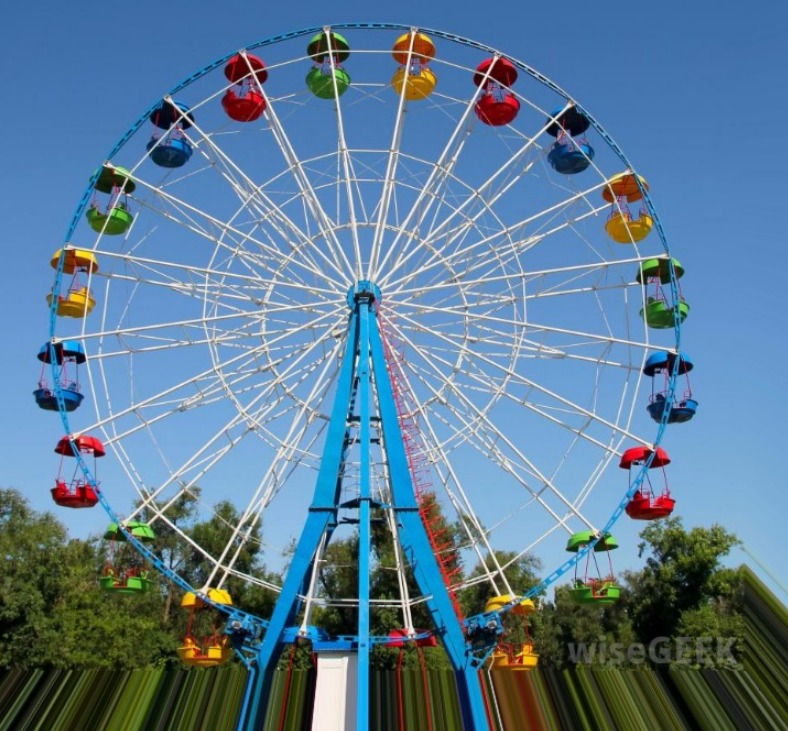
\includegraphics[width=\textwidth,height=0.62\textheight,keepaspectratio]{rueda.jpeg}%
				}{%
					\imgwarning{rueda de la fortuna (ferris wheel)}%
				}%
			}
		\end{column}
		\begin{column}{0.5\textwidth}
			\centering
			\IfFileExists{imagenes/rusa.jpeg}{%
				\includegraphics[width=\textwidth,height=0.62\textheight,keepaspectratio]{imagenes/rusa.jpeg}%
			}{%
				\IfFileExists{rusa.jpeg}{%
					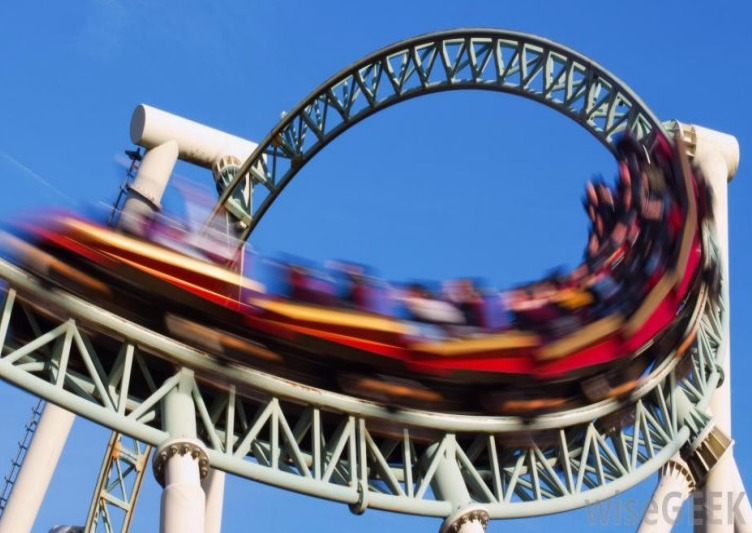
\includegraphics[width=\textwidth,height=0.62\textheight,keepaspectratio]{rusa.jpeg}%
				}{%
					\imgwarning{montaña rusa con curva circular (roller coaster loop)}%
				}%
			}
		\end{column}
	\end{columns}
	\vspace{0.3cm}
	\begin{center}
		\small Dos ejemplos cotidianos de movimiento (aproximadamente) circular.
	\end{center}
\end{frame}
	
	% ============================================================
	% SLIDE 13: RELACIÓN COORDENADAS ANGULARES Y LINEALES
	% ============================================================
	\begin{frame}{Relación Coordenadas Angulares y Lineales}
		\renewcommand{\arraystretch}{2.0}
		\begin{center}
			\begin{tabular}{cc}
				\toprule
				\textbf{Cinemática Lineal} & \textbf{Cinemática Rotacional} \\
				\midrule
				$a = \text{cte}$ & $\alpha = \text{cte}$ \\
				$v = a\,\Delta t + v_0$ & $\omega = \alpha\,\Delta t + \omega_0$ \\
				$x = \dfrac{1}{2}a(\Delta t)^2 + v_0\,\Delta t + x_0$ &
				$\theta = \dfrac{1}{2}\alpha(\Delta t)^2 + \omega_0\,\Delta t + \theta_0$ \\
				\bottomrule
			\end{tabular}
		\end{center}
		\vspace{0.3cm}
		\small La analogía es exactamente la misma que vimos en la Sesión 2 para $x,v,a$ con aceleración constante: \textbf{basta reemplazar $x\to\theta$, $v\to\omega$, $a\to\alpha$.}
	\end{frame}
	
	% ============================================================
	% SLIDE 14: MCU -- DEFINICIONES
	% ============================================================
\begin{frame}{Movimiento Circular Uniforme}
	\begin{center}
		\IfFileExists{rueda.jpeg}{%
			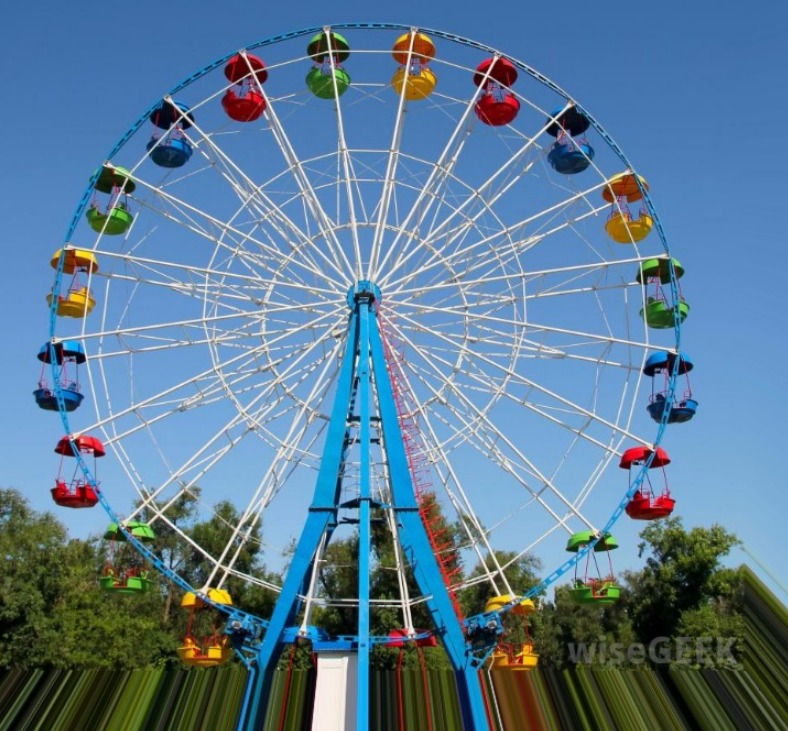
\includegraphics[width=0.95\textwidth,height=0.4\textheight,keepaspectratio]{rueda.jpeg}%
		}{%
			\IfFileExists{imagenes/rueda.jpeg}{%
				\includegraphics[width=0.45\textwidth,height=0.4\textheight,keepaspectratio]{imagenes/rueda.jpeg}%
			}{%
				\imgwarning[0.45]{rueda de la fortuna (ferris wheel)}%
			}%
		}
	\end{center}
	\[
	|\vec r| = r = \text{cte} \quad\to\quad \text{Movimiento en círculo}
	\]
	\[
	\omega = \frac{d\theta}{dt} = \text{cte} \quad\to\quad \text{Velocidad angular (rad/s)}
	\]
\end{frame}
	
	% ============================================================
	% SLIDE 15: MCU -- VELOCIDAD Y ACELERACIÓN
	% ============================================================
\begin{frame}{Movimiento Circular Uniforme}
	\begin{columns}[T]
		\begin{column}{0.5\textwidth}
			\centering
			\begin{tikzpicture}[scale=1.15]
				\draw[thick] (0,0) circle (2);
				\foreach \ang in {90,210,330} {
					\filldraw[fill=blue!25, draw=blue!70!black] (\ang:2) circle (2.8pt);
					\draw[very thick, magenta, -{Latex}] (\ang:2) -- ($(\ang:2)+(\ang+90:1.0)$);
					\draw[very thick, orange!90!black, -{Latex}] (\ang:2) -- ($(\ang:2)+(\ang+180:0.9)$);
					% etiqueta v: desplazada en la direccion tangencial
					\node[magenta, font=\small] at ($(\ang:2)+(\ang+90:1.35)$) {$\vec v$};
					% etiqueta a: desplazada radialmente hacia adentro (un poco mas alla del vector)
					\node[orange!90!black, font=\small] at ($(\ang:2)+(\ang+180:1.25)$) {$\vec a$};
				}
			\end{tikzpicture}
		\end{column}
		\begin{column}{0.5\textwidth}
			\[
			|\vec v| = v = \text{cte}, \quad \vec v = r\omega\,\hat\theta
			\]
			\small $\to$ tangente al camino: velocidad lineal o tangencial.
			\[
			|\vec a| = a = \text{cte}, \quad \vec a = -r\omega^2\,\hat r
			\]
			\small $\to$ apunta hacia el centro: \textbf{\textcolor{red}{Aceleración Centrípeta}}.
		\end{column}
	\end{columns}
\end{frame}
	
	% ============================================================
	% SLIDE 16: EJEMPLO -- ACELERACIÓN CENTRÍPETA DE LA TIERRA
	% ============================================================
\begin{frame}{Ej: Aceleración Centrípeta de la Tierra}
	Aproxime que la Tierra se mueve en una órbita circular alrededor del Sol. Calcule la magnitud de su aceleración centrípeta si el radio de la órbita es $1.496\times10^{11}$ m.
	\[
	a_c = \frac{v^2}{r} = \omega^2 r, \qquad \omega = \frac{2\pi}{T}
	\]
	\[
	\to a_c = r\left(\frac{2\pi}{T}\right)^2 = 1.496\times10^{11}\text{ m}\times\left(\frac{2\pi}{365\times24\times3600\text{ s}}\right)^2
	\]
	\[
	\to a_c \approx 5.94\times10^{-3}\text{ m/s}^2
	\]
	\small\textit{Dirección: hacia el Sol ($-\hat r$), consistente con una aceleración centrípeta.}
\end{frame}
	
	% ============================================================
	% SLIDE 17: EJEMPLO -- POLEA
\begin{frame}{Ejemplo}
	Un hombre hace girar la polea del dibujo a 10 rev/min. Si la polea tiene un diámetro de 15 cm: a) ¿Cuál es su velocidad angular? b) ¿Qué ángulo ha barrido al cabo de 10 s?
	\begin{columns}[T]
		\begin{column}{0.4\textwidth}
			\centering
			\IfFileExists{polea.jpeg}{%
				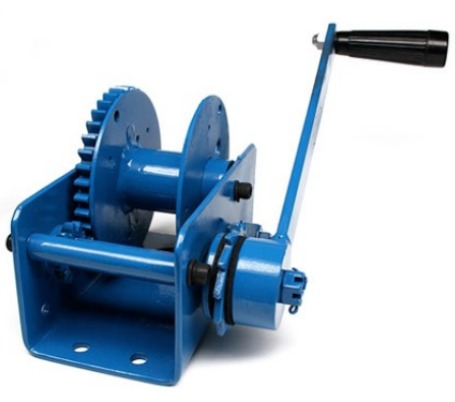
\includegraphics[width=\textwidth,height=0.6\textheight,keepaspectratio]{polea.jpeg}%
			}{%
				\IfFileExists{imagenes/polea.jpeg}{%
					\includegraphics[width=\textwidth,height=0.6\textheight,keepaspectratio]{imagenes/polea.jpeg}%
				}{%
					\imgwarning[1.0]{manivela/polea manual (hand crank winch)}%
				}%
			}
		\end{column}
		\begin{column}{0.6\textwidth}
			\textbf{a)} 
			\[
			\omega = 2\pi f = 2\pi\text{ rad}\times\frac{10\text{ rev}}{60\text{ s}} = 1.047\ \frac{\text{rad}}{\text{s}}
			\]
			\textbf{b)}
			\[
			\theta = \omega t = 1.047\ \frac{\text{rad}}{\text{s}}\times 10\text{ s} = 10.47\text{ rad}
			\]
		\end{column}
	\end{columns}
\end{frame}
	
	% ============================================================
	% SLIDE 18: MCU -- DERIVACIÓN theta(t)
	% ============================================================
	\begin{frame}{Movimiento Circular Uniforme}
		Al igual que hicimos en la Sesión 2 para la velocidad, integramos $\omega = \text{cte}$ para obtener $\theta(t)$:
		\[
		\omega = \frac{d\theta}{dt}
		\]
		\[
		\to \omega\int_{t_0}^{t} dt' = \int_{\theta_0}^{\theta(t)} d\theta'
		\]
		\[
		\to \omega(t-t_0) = \theta(t) - \theta_0
		\]
		\[
		\boxed{\theta(t) = \theta_0 + \omega(t-t_0)}
		\]
	\end{frame}
	
	% ============================================================
	% SLIDE 19: MCU -- PARAMETRIZACIÓN x(t), y(t)
\begin{frame}{Movimiento Circular Uniforme}
	\begin{columns}[T]
		\begin{column}{0.45\textwidth}
			\centering
			\begin{tikzpicture}[scale=1.15]
				\draw (0,0) circle (2);
				\draw[->] (-2.4,0) -- (2.6,0) node[right]{\normalsize $x$};
				\draw[->] (0,-2.4) -- (0,2.6) node[above]{\normalsize $y$};
				% Vector posicion
				\draw[very thick, -{Latex}] (0,0) -- (35:2) node[midway, above left]{\small $\vec r$};
				% Punto del objeto sobre la circunferencia
				\filldraw[UnalGreen] (35:2) circle (3.5pt);
				% Proyecciones
				\draw[dashed] (35:2) -- (0,{2*sin(35)});
				\node[left, font=\small] at (0,{2*sin(35)}) {$y(t)$};
				\draw[dashed] (35:2) -- ({2*cos(35)},0);
				\node[below, font=\small] at ({2*cos(35)},-0.05) {$x(t)$};
				% Angulo theta
				\draw (0.6,0) arc(0:35:0.6);
				\node[font=\small] at (17.5:0.95) {$\theta(t)$};
				% Flecha de omega, ahora en sentido antihorario
				\draw[->, thick] (110:2.35) arc (110:140:2.35);
				\node[font=\small] at (125:2.65) {$\omega$};
				\node[below left, font=\small] at (0,0) {$O$};
			\end{tikzpicture}
		\end{column}
		\begin{column}{0.55\textwidth}
			\[
			x(t) = r\cos\omega t, \qquad y(t) = r\sin\omega t
			\]
			\[
			\to x^2+y^2 = r^2\cos^2\omega t + r^2\sin^2\omega t
			\]
			\[
			\to \boxed{x^2+y^2 = r^2}
			\]
			\small (confirma que la trayectoria es, en efecto, un círculo de radio $r$).
		\end{column}
	\end{columns}
\end{frame}
	
	% ============================================================
	% SLIDE 20: EJEMPLO 1 -- theta(t) (enunciado + graf)
	% ============================================================
	\begin{frame}{Movimiento Circular Uniforme}
		\small Ejemplo 1: La figura muestra la posición angular de un punto pintado sobre la orilla de una rueda rotante. Describa el movimiento de la rueda en una gráfica de $\omega$ vs. $t$.
		\begin{columns}[T]
			\begin{column}{0.55\textwidth}
				\centering
				\begin{tikzpicture}[x=0.9cm, y=0.26cm]
					\draw[->] (0,0) -- (6.6,0) node[right]{\small $t$ (s)};
					\draw[->] (0,-1) -- (0,20) node[above]{\small $\theta$ (rad)};
					\foreach \tk in {1,2,3,4,5,6} \draw (\tk,-0.5)--(\tk,0.5) node[below=2pt]{\tiny \tk};
					\node[left] at (0,18.85){\tiny $6\pi$};
					\node[left] at (0,12.57){\tiny $4\pi$};
					\draw[gray!50,dashed] (0,18.85) -- (3,18.85);
					\draw[gray!50,dashed] (0,12.57) -- (6.3,12.57);
					\draw[thick, UnalGreen] (0,0) -- (3,18.85) -- (5,12.57) -- (6.3,12.57);
					\node at (1.3,9) {\footnotesize 1};
					\node at (4.15,16.7) {\footnotesize 2};
					\node at (5.7,13.8) {\footnotesize 3};
				\end{tikzpicture}
			\end{column}
			\begin{column}{0.45\textwidth}
				\footnotesize
				\begin{itemize}
					\item En 1: $\omega = \dfrac{6\pi\text{ rad}}{3\text{ s}} = 2\pi$ rad/s
					\item En 2: $\omega = \dfrac{(4\pi-6\pi)\text{ rad}}{(5-3)\text{ s}} = -\pi$ rad/s
					\item En 3: $\omega = 0$ rad/s
				\end{itemize}
				\[
				\theta(t) = \theta_0 + \omega t - \omega t_0
				\]
			\end{column}
		\end{columns}
	\end{frame}
	
	% ============================================================
	% SLIDE 21: EJEMPLO 1 -- ambas gráficas
	% ============================================================
\begin{frame}{Movimiento Circular Uniforme}
	\small La figura muestra la posición angular de un punto pintado sobre la orilla de una rueda rotante. Describa el movimiento de la rueda en una gráfica de $\omega$ vs. $t$.
	\begin{columns}[T]
		\begin{column}{0.5\textwidth}
			\centering
			\begin{tikzpicture}[x=0.9cm, y=0.27cm]
				\draw[->] (0,0) -- (6.6,0) node[right]{\small $t$ (s)};
				\draw[->] (0,-1) -- (0,20) node[above]{\small $\theta$ (rad)};
				\foreach \tk in {1,2,3,4,5,6} \draw (\tk,-0.5)--(\tk,0.5) node[below=2pt]{\small \tk};
				\node[left, font=\small] at (0,18.85) {$6\pi$};
				\node[left, font=\small] at (0,12.57) {$4\pi$};
				\draw[thick, UnalGreen] (0,0) -- (3,18.85) -- (5,12.57) -- (6.3,12.57);
			\end{tikzpicture}
		\end{column}
		\begin{column}{0.5\textwidth}
			\centering
			\begin{tikzpicture}[x=0.9cm, y=0.5cm]
				\draw[->] (0,-4.5) -- (0,7) node[above]{\small $\omega$ (rad/s)};
				\draw[->] (-0.3,0) -- (6.6,0) node[right]{\small $t$ (s)};
				\foreach \tk in {1,2,3,4,5,6} \draw (\tk,-0.2)--(\tk,0.2) node[below=1pt]{\small \tk};
				\node[left, font=\small] at (0,6.283) {$2\pi$};
				\node[left, font=\small] at (0,-3.1416) {$-\pi$};
				\draw[thick, UnalGreen] (0,6.283) -- (3,6.283);
				\draw[thick, UnalGreen, dashed] (3,6.283) -- (3,-3.1416);
				\draw[thick, UnalGreen] (3,-3.1416) -- (5,-3.1416);
				\draw[thick, UnalGreen, dashed] (5,-3.1416) -- (5,0);
				\draw[thick, UnalGreen] (5,0) -- (6.3,0);
				\node[font=\small] at (1.4,7) {1};
				\node[font=\small] at (4,-4) {2};
				\node[font=\small] at (5.7,0.7) {3};
			\end{tikzpicture}
		\end{column}
	\end{columns}
\end{frame}
	
	% ============================================================
	% SLIDE 22: RECURSOS
	% ============================================================
	\begin{frame}{Recursos Interactivos}
		\begin{block}{Simulador de rotación (PhET)}
			\url{https://phet.colorado.edu/en/simulation/rotation}
		\end{block}
	\end{frame}
	
	% ============================================================
	% SLIDE 18 (ORIGINAL): CIERRE
	% ============================================================
	\begin{frame}{Cierre de la sesión}
		\begin{columns}[T]
			\begin{column}{0.5\textwidth}
				\begin{block}{Lo esencial de hoy}
					\small
					\begin{itemize}
						\item $\theta = \dfrac{s}{r}, \quad \omega = \dfrac{d\theta}{dt} = \dfrac{2\pi}{T} = 2\pi f$
						\item MCU: $v = r\omega$ (tangencial, $\hat\theta$)
						\item Aceleración centrípeta: $a = r\omega^2$ (hacia el centro, $-\hat r$)
						\item Analogía lineal $\leftrightarrow$ rotacional: $x\to\theta,\ v\to\omega,\ a\to\alpha$
					\end{itemize}
				\end{block}
				
				\vspace{0.25cm}
				\begin{exampleblock}{Próximamente}
					\small
					El \textbf{Taller de Movimiento Circular} se publicará en Classroom para la próxima sesión.
				\end{exampleblock}
			\end{column}
			\begin{column}{0.5\textwidth}
				\begin{center}
					\vspace{0.3cm}
					\Large \textbf{¿Preguntas?}
					
					\vspace{0.8cm}
					\normalsize
					Nos vemos la próxima sesión.
					
					\vspace{0.6cm}
					mperdomog@unal.edu.co
					
					\vspace{0.2cm}
					Edificio 401 -- Salón 202
				\end{center}
			\end{column}
		\end{columns}
	\end{frame}
	
\end{document}